\documentclass[12pt]{article}

\usepackage{amsmath, amssymb}
\usepackage{physics}
\usepackage{graphicx}
\usepackage{tikz}
\usepackage{siunitx}
\usepackage{tcolorbox}
\usepackage{geometry}
\geometry{margin=1in}

\title{Physics 122 --- Thermal Physics}
\author{Lecture Notes: Week 3, Day 3}
\date{}

\begin{document}
\maketitle

%------------------------------------------------
\section{Adiabatic Processes}

\begin{tcolorbox}[colback=gray!10,title=Definition]
An \textbf{adiabatic process} is a thermodynamic process in which \textbf{no heat is exchanged} with the surroundings:
\[
Q = 0
\]
\end{tcolorbox}

\subsection{First Law of Thermodynamics (Course Convention)}

\begin{tcolorbox}[colback=blue!5]
\textbf{Sign convention:}  
Work done \emph{by the environment on the system} is positive.
\end{tcolorbox}

\[
\boxed{\Delta E = Q + W}
\]

For an adiabatic process:
\[
\boxed{\Delta E = W}
\]

\subsection{Physical Examples}
\begin{itemize}
  \item Opening a soda bottle (rapid gas expansion)
  \item Spraying deodorant
  \item Diesel engine compression (no spark plug)
\end{itemize}

Rapid expansion or compression occurs too quickly for heat transfer.

\subsection{Temperature Change}
\begin{itemize}
  \item Expansion $\rightarrow W<0 \rightarrow$ internal energy decreases $\rightarrow$ gas cools
  \item Compression $\rightarrow W>0 \rightarrow$ internal energy increases $\rightarrow$ gas heats
\end{itemize}

%------------------------------------------------
\section{Adiabatic vs Isothermal Processes}

\subsection{Ideal Gas Law}
\[
PV = nRT
\]

\subsection{Isothermal Process}
\[
T = \text{constant}, \qquad P = \frac{nRT}{V}
\]

\subsection{Adiabatic Process}
\[
\boxed{PV^\gamma = \text{constant}}
\]
where
\[
\gamma = \frac{C_P}{C_V}
\]


\begin{center}
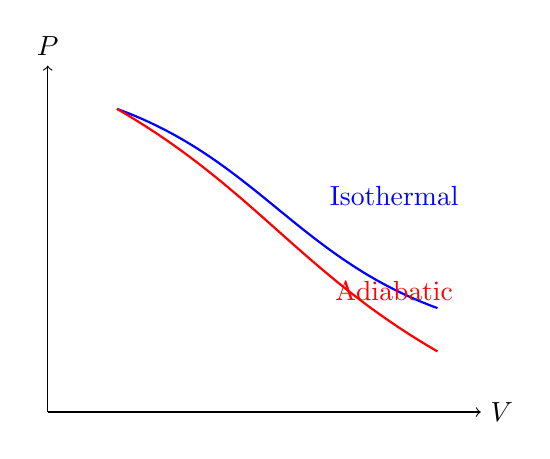
\begin{tikzpicture}[scale=1.1]
  \draw[->] (0,0) -- (5,0) node[right] {$V$};
  \draw[->] (0,0) -- (0,4) node[above] {$P$};

  % Isothermal
  \draw[thick, blue] (0.8,3.5) to[out=-20,in=160] (4.5,1.2);
  \node[blue] at (4,2.5) {Isothermal};

  % Adiabatic
  \draw[thick, red] (0.8,3.5) to[out=-30,in=150] (4.5,0.7);
  \node[red] at (4,1.4) {Adiabatic};
\end{tikzpicture}
\end{center}


Adiabatic curves are steeper than isothermal curves.

%------------------------------------------------
\section{Thermal Expansion}

\subsection{Linear Expansion}

\begin{tcolorbox}[colback=gray!10,title=Linear Expansion]
\[
\boxed{\Delta L = \alpha L_0 \Delta T}
\]
\end{tcolorbox}

\begin{itemize}
  \item $\alpha$ has units of \(\si{K^{-1}}\)
  \item Depends on material
\end{itemize}

\subsection{Volume Expansion}
\[
\boxed{\Delta V = \beta V_0 \Delta T}
\]

For isotropic solids:
\[
\boxed{\beta \approx 3\alpha}
\]

\subsection{Microscopic Picture}

\begin{center}
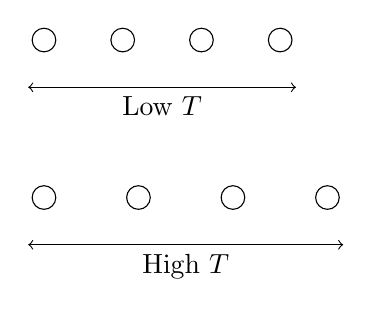
\begin{tikzpicture}
  \foreach \x in {0,1,2,3} {
    \draw (\x,0) circle (0.15);
  }
  \draw[<->] (-0.2,-0.6) -- (3.2,-0.6) node[midway,below] {Low $T$};

  \foreach \x in {0,1.2,2.4,3.6} {
    \draw (\x,-2) circle (0.15);
  }
  \draw[<->] (-0.2,-2.6) -- (3.8,-2.6) node[midway,below] {High $T$};
\end{tikzpicture}
\end{center}

Higher temperature increases atomic vibration amplitude, increasing average spacing.

%------------------------------------------------
\section{Example: Warming a Frozen Popsicle}

\textbf{Problem:}  
A \SI{50}{g} popsicle is removed from a freezer at \(-10^\circ\text{C}\) and warmed to \(20^\circ\text{C}\).

\textbf{Given:}
\[
c_{\text{ice}} = \SI{2100}{J/(kg\cdot K)}
\]
\[
c_{\text{water}} = \SI{4200}{J/(kg\cdot K)}
\]
\[
L_f = 3\times10^5\,\si{J/kg}
\]

\subsection*{Steps}
\begin{align*}
Q_1 &= m c_{\text{ice}} (0 - (-10)) \\
Q_2 &= m L_f \\
Q_3 &= m c_{\text{water}} (20 - 0)
\end{align*}

\subsection*{Total Heat}
\[
\boxed{Q = Q_1 + Q_2 + Q_3 \approx 1.93\times10^4\,\text{J}}
\]

%------------------------------------------------
\end{document}